\documentclass[11pt,oneside,a4paper]{book}
\usepackage[%
  a4paper,%
  left = 20mm,%
  right = 20mm,%
  textwidth = 178mm,%
  top = 40mm,%
  bottom = 30mm,%
  %heightrounded,%
  headheight=70pt,%
  headsep=25pt,%
]{geometry}
\usepackage{graphicx}
\usepackage[sfdefault,light]{FiraSans}
\usepackage{hyperref}
\hypersetup{
    colorlinks = true,
    allcolors  = link-blue, 
}
\usepackage{lastpage}
\usepackage{graphicx}
\usepackage{float}
\usepackage{xspace}
\usepackage{longtable}
\usepackage{tabularx}
\usepackage{color,colortbl}
\usepackage{longtable} % Paquete para tablas largas
\usepackage{colortbl}  % Colores en tablas
\usepackage[table,xcdraw]{xcolor} % Colores adicionales


\definecolor{link-blue}{RGB}{6,69,173}
\definecolor{dark-green}{RGB}{52,133,62}
\definecolor{light-blue}{RGB}{127,180,240}
\definecolor{dark-blue}{RGB}{72,120,224}
\definecolor{heading-grey}{RGB}{128,128,128}
\definecolor{heading2-grey}{RGB}{200,200,200}
\definecolor{Critical}{RGB}{192,0,0}
\definecolor{High}{RGB}{255,0,0}
\definecolor{Medium}{RGB}{255,192,0}
\definecolor{Low}{RGB}{255,255,0}
\definecolor{Informational}{RGB}{94,185,255}

\usepackage{listings}
\usepackage{enumitem}
\usepackage{array,booktabs}
\usepackage{fancyhdr}
\renewcommand{\footrulewidth}{0.2pt}
\renewcommand{\headrulewidth}{0.2pt}
\fancyfoot{}
\fancyhead{}
\fancyfoot[C]{Confidential}
\fancypagestyle{plain}{
    \fancyfoot[R]{\\ \textcolor{heading-grey}{\newline Página \thepage\ de \pageref{LastPage}}}
    \fancyfoot[C]{\textcolor{heading-grey}{\textbf{Clase HE 24/25 -- \projectno}  }}
    \fancyhead[R]{
\includegraphics[width=1cm]{img/logo.jpg}}
}
\fancypagestyle{fancy}{
    \fancyfoot[R]{\\ \textcolor{heading-grey}{\newline Página \thepage\ de \pageref{LastPage}}}
    \fancyfoot[C]{\textcolor{heading-grey}{\textbf{Clase HE 24/25 -- \projectno}   }}
    \fancyhead{}
}
\thispagestyle{fancy}\pagestyle{plain}

\newcommand{\email}[1]{\href{mailto://#1}{#1}}
\newcommand{\newchapter}[1]{{\section*{#1}
\addcontentsline{toc}{chapter}{#1}}}
\newcommand{\newsection}[1]{{\subsection*{#1}
\addcontentsline{toc}{section}{#1}}}
\newcommand{\newsubsection}[1]{{\subsubsection*{#1}
\addcontentsline{toc}{subsection}{#1}}}
\usepackage[skip=10pt plus1pt, indent=0pt]{parskip}
\usepackage{float} % Añadir al preámbulo si no lo tienes

\usepackage{etoolbox}
\makeatletter
\patchcmd{\chapter}{\if@openright\cleardoublepage\else\clearpage\fi}{}{}{}
\makeatother
\makeatletter
\renewcommand\tableofcontents{%
    \if@twocolumn
      \@restonecoltrue\onecolumn
    \else
      \@restonecolfalse
    \fi
    \section*{\contentsname
        \@mkboth{%
           \MakeUppercase\contentsname}{\MakeUppercase\contentsname}}%
    \@starttoc{toc}%
    \if@restonecol\twocolumn\fi
    }
\makeatother

\usepackage{titlesec}

\titleformat{\section}
{\normalfont\huge\bfseries}{\thesection}{1em}{}
\titleformat{\subsection}
{\normalfont\Large\bfseries}{\thesubsection}{1em}{}
\titleformat{\subsubsection}
{\normalfont\large\bfseries}{\thesubsubsection}{1em}{}

% \titleformat{command}[shape]{format}{label}{sep}{before}[after]
% \titlespacing{command}{left spacing}{before spacing}{after spacing}[right]

\titlespacing{\section}{0pt}{1em}{0.5em}
\titlespacing{\subsection}{0pt}{0em}{0.25em}

\usepackage[T1]{fontenc}
\renewcommand*\oldstylenums[1]{{\firaoldstyle #1}}

\def\projectno{100-01}


\usepackage[spanish]{babel}
\usepackage[utf8]{inputenc}
\usepackage[T1]{fontenc}

\begin{document}

\renewcommand{\headrulewidth}{0pt}

%%%%%%%%%%%%%%%%%%%%%%%%%%%%%%%%%%%%%%%%%
%%          Begin title page           %%
%%%%%%%%%%%%%%%%%%%%%%%%%%%%%%%%%%%%%%%%%

\begin{titlepage}
   \thispagestyle{fancy}
   \begin{center}
        \vspace*{8em}
   
        \centering
\includegraphics[width=13cm]{img/logo_iescierva.jpg}

        \vspace{3em}

        \huge{\textbf{Clase HE 24/25 \\
        Informe de resultados de la evaluación de la seguridad \\
        Metasploitable 2}}

        \vspace{10em}

   \end{center}

    \normalsize{Fecha: \today \\
    Proyecto: \projectno \\
    Version 1.0}
\end{titlepage}

\renewcommand{\headrulewidth}{0.2pt}

\newpage

\tableofcontents

\newpage

%%%%%%%%%%%%%%%%%%%%%%%%%%%%%%%%%%%%%%%%%
%%           Begin contents            %%
%%%%%%%%%%%%%%%%%%%%%%%%%%%%%%%%%%%%%%%%%

\newchapter{Información de contacto}

\begin{table}[h]
\begin{center}
    \begin{tabular}{|m{4cm}|m{4cm}|m{7.5cm}|} % Anchos ajustados aquí
        \hline
        \rowcolor{heading-grey}\multicolumn{1}{|>{\centering\arraybackslash}m{4cm}|}{\textcolor{white}{\textbf{Nombre}}} & 
        \multicolumn{1}{>{\centering\arraybackslash}m{4cm}|}{\textcolor{white}{\textbf{Título}}} & 
        \multicolumn{1}{>{\centering\arraybackslash}m{7.5cm}|}{\textcolor{white}{\textbf{Contacto}}} \\ \hline
        José María Alcaraz & Docente / Principal & Email: \href{mailto:josemaria.alcaraz2@murciaeduca.es}{josemaria.alcaraz2@murciaeduca.es} \\ \hline
    \end{tabular}
\end{center}
\end{table}


\newpage

\newchapter{Antecedentes}

El pasado 11 de diciembre de 2024, durante una sesión de clase de Hacking Ético, asigné a mis alumnos la tarea de realizar su primera auditoría de seguridad en un lapso aproximado de 3 horas. Tras recibir sus reportes a través de la plataforma Moodle, ahora procederé, como docente, a presentar mi propia auditoría realizada bajo las mismas condiciones de tiempo.

Para hacer más realista dicha auditoría, vamos a suponer que es para un cliente. El cliente solicita ayuda a los participantes de la clase de Hacking Ético en el instituto Ingeniero de la Cierva 2024/2025 debido a un fallo de seguridad detectado en una de sus máquinas. Según indica, se trata de una máquina virtual antigua que pertenecía al anterior informático de la empresa. Desde que esta persona dejó su puesto, nadie la ha actualizado ni sabe cómo acceder a ella, ya que actualmente no tienen personal informático en plantilla. 

El único dato que poseen es la dirección IP de la máquina. Al parecer, el cliente tiene indicios de que alguien podría haber accedido a dicha máquina sin autorización, pero desconoce cómo se ha producido dicho acceso. Por ello, solicita a los participantes de la clase que realicen una auditoría de seguridad de la máquina virtual e intenten identificar las posibles vías de acceso utilizadas por los atacantes.


\newchapter{Fases de la auditoria}

Las fases de las actividades de pruebas de penetración incluyen las siguientes:

\begin{itemize}
    \item \textbf{Planificación} -- Se recopilan los objetivos del cliente y se obtienen las reglas de compromiso.
    \item \textbf{Descubrimiento} -- Se realizan análisis y enumeración para identificar posibles vulnerabilidades, áreas débiles y exploits.
    \item \textbf{Ataque} -- Se confirman las vulnerabilidades potenciales a través de la explotación y se realiza un descubrimiento adicional tras obtener nuevos accesos.
    \item \textbf{Reporte} -- Se documentan todas las vulnerabilidades y exploits encontrados, los intentos fallidos y las fortalezas y debilidades de la empresa.
\end{itemize}

\newpage

\newchapter{Calificación de la gravedad}

La siguiente tabla define los niveles de gravedad y el rango de puntuación CVSS correspondiente que se utilizan a lo largo del documento para evaluar las vulnerabilidades y el impacto del riesgo.

\begin{table}[h]
    \begin{center}
        \begin{tabular}{|m{3cm}|m{2.5cm}|m{10cm}|}
        \hline
        \rowcolor{heading-grey}\multicolumn{1}{|>{\centering\arraybackslash}m{30mm}|}{\textcolor{white}{\textbf{Gravedad}}} & 
        \multicolumn{1}{>{\centering\arraybackslash}m{25mm}|}{\textcolor{white}{\textbf{Rango de puntuación CVSS V3}}} & 
        \multicolumn{1}{>{\centering\arraybackslash}m{100mm}|}{\textcolor{white}{\textbf{Definición}}} \\ \hline
        % Begin security ratings %
        \cellcolor{Critical}\textbf{\textcolor{white}{Crítica}} & \centering 9.0 -- 10.0 & La explotación es directa y, por lo general, resulta en un compromiso a nivel de sistema. Se recomienda crear un plan de acción y aplicar parches de inmediato. \\ \hline
        \cellcolor{High}\textbf{Alta} & \centering 7.0 -- 8.9 & La explotación es más difícil pero podría ocasionar privilegios elevados y, potencialmente, la pérdida de datos o interrupciones en el servicio. Se recomienda crear un plan de acción y aplicar parches lo antes posible. \\ \hline
        \cellcolor{Medium}\textbf{Moderada} & \centering 4.0 -- 6.9 & Existen vulnerabilidades, pero no son explotables directamente o requieren pasos adicionales, como ingeniería social. Se recomienda crear un plan de acción y aplicar parches después de resolver los problemas de alta prioridad. \\ \hline
        \cellcolor{Low}\textbf{Baja} & \centering 0.1 -- 3.9 & Las vulnerabilidades no son explotables, pero aumentan la superficie de ataque de la organización. Se recomienda crear un plan de acción y aplicar parches durante la próxima ventana de mantenimiento. \\ \hline
        \cellcolor{Informational}\textbf{Informativa} & \centering N/A & No existe vulnerabilidad conocida. Se proporciona información adicional sobre elementos observados durante la prueba, controles robustos y documentación adicional. \\ \hline
\end{tabular}
    \end{center}
\end{table}


\newchapter{Alcance}

\newsection{Exclusiones del alcance}

El cliente especificó que no se debían crear, modificar ni eliminar ningún archivo o carpeta del servidor.

\newsection{Permisos otorgados}

No se proporcionaron permisos especiales para ayudar en la realización de la auditoría.

\newsection{Información adicional proporcionada}
El cliente nos proporciona la siguiente dirección IP: 192.168.56.101

\newpage
\newchapter{Planificación}

La fase de planificación es esencial para garantizar que la auditoría de seguridad se realice de manera controlada y cumpliendo con los objetivos definidos por el cliente. En este caso, como parte del escenario simulado en el contexto de la clase de Hacking Ético, se establecieron los siguientes objetivos y reglas de compromiso:

\begin{itemize}
    \item \textbf{Objetivos del cliente:}  
    El cliente ficticio, representado por una empresa que opera sin personal técnico en plantilla, planteó un problema relacionado con una máquina virtual antigua que había quedado desatendida desde la salida de su último informático. El principal objetivo de la auditoría es identificar posibles vulnerabilidades que permitan o hayan permitido accesos no autorizados, comprender cómo se pudo haber comprometido dicha máquina y proporcionar recomendaciones claras para mitigar los riesgos identificados. 

    \item \textbf{Contexto del cliente:}  
    La máquina virtual en cuestión no ha sido actualizada ni gestionada durante un periodo prolongado. El único dato proporcionado por el cliente es la dirección IP de la máquina, ya que no cuentan con credenciales ni documentación adicional. Esto refleja un escenario realista donde los auditores deben trabajar con información limitada y depender de técnicas de descubrimiento y enumeración.

    \item \textbf{Reglas de compromiso:}  
    El cliente especificó explícitamente las siguientes restricciones:
    \begin{itemize}
        \item No crear, modificar ni eliminar ningún archivo o carpeta en la máquina virtual.
        \item No realizar ataques destructivos, como pruebas de Denegación de Servicio (DoS).
        \item Limitar el tiempo de la auditoría a un máximo de 3 horas.
    \end{itemize}
    Estas reglas aseguran que la auditoría se realice de forma controlada y que no se comprometa la integridad de los sistemas evaluados.

    \item \textbf{Preparativos:}  
    Antes de iniciar la auditoría, se definió un plan de acción detallado que incluye las herramientas y técnicas a utilizar. Entre ellas:
    \begin{itemize}
        \item Herramientas para escaneo de red y enumeración de servicios, como \texttt{nmap}.
        \item Herramientas de análisis de vulnerabilidades para evaluar los servicios detectados.
        \item Herramientas de explotación de vulnerabilidades, como \texttt{metasploit}
    \end{itemize}
    Además, se estableció un flujo de trabajo claro para registrar todas las actividades realizadas, documentar cualquier vulnerabilidad identificada y garantizar que el análisis fuera replicable.

    \item \textbf{Alcance temporal:}  
    Se asignó un tiempo máximo de 3 horas para completar la auditoría, incluyendo las fases de descubrimiento, análisis y documentación inicial.
\end{itemize}

En esta etapa, se dejó claro que el propósito principal de la auditoría no era únicamente identificar vulnerabilidades, sino también proporcionar a los participantes un enfoque práctico y controlado de cómo realizar un análisis de seguridad estructurado en un entorno profesional.


\newpage

\newchapter{Descubrimiento}
Debido a la limitación de tiempo, es posible que la fase de descubrimiento esté incompleta.
\newsection{Puertos abiertos}
\begin{lstlisting}[language=bash, caption=Comando Nmap usado]
nmap -sS -sV -O -T3 --top-ports 1000 --reason --open 192.168.56.101
\end{lstlisting}

\begin{table}[H]
\renewcommand{\arraystretch}{1.3}
\small
\begin{center}
\begin{tabular}{|p{1.5cm}|p{2cm}|p{4cm}|p{5.5cm}|}
\hline
\rowcolor{heading-grey}
\textbf{\textcolor{white}{Puerto}} & \textbf{\textcolor{white}{Estado}} & \textbf{\textcolor{white}{Servicio}} & \textbf{\textcolor{white}{Detalles}} \\ \hline

21/tcp & Abierto & FTP & vsftpd 2.3.4 \\ \hline
22/tcp & Abierto & SSH & OpenSSH 4.7p1 Debian 8ubuntu1 (protocol 2.0) \\ \hline
23/tcp & Abierto & Telnet & Linux telnetd \\ \hline
25/tcp & Abierto & SMTP & Postfix smtpd \\ \hline
53/tcp & Abierto & DNS & ISC BIND 9.4.2 \\ \hline
80/tcp & Abierto & HTTP & Apache httpd 2.2.8 ((Ubuntu) DAV/2) \\ \hline
111/tcp & Abierto & RPCbind & Versión 2 (RPC \#100000) \\ \hline
139/tcp & Abierto & NetBIOS-SSN & Samba smbd 3.X - 4.X (workgroup: WORKGROUP) \\ \hline
445/tcp & Abierto & NetBIOS-SSN & Samba smbd 3.X - 4.X (workgroup: WORKGROUP) \\ \hline
512/tcp & Abierto & Exec & netkit-rsh rexecd \\ \hline
513/tcp & Abierto & Login & OpenBSD o Solaris rlogind \\ \hline
514/tcp & Abierto & Shell & Netkit rshd \\ \hline
1099/tcp & Abierto & Java-RMI & GNU Classpath grmiregistry \\ \hline
1524/tcp & Abierto & Bind Shell & Metasploitable root shell \\ \hline
2049/tcp & Abierto & NFS & Versiones 2-4 (RPC \#100003) \\ \hline
2121/tcp & Abierto & FTP & ProFTPD 1.3.1 \\ \hline
3306/tcp & Abierto & MySQL & MySQL 5.0.51a-3ubuntu5 \\ \hline
5432/tcp & Abierto & PostgreSQL & PostgreSQL DB 8.3.0 - 8.3.7 \\ \hline
5900/tcp & Abierto & VNC & VNC (protocolo 3.3) \\ \hline
6000/tcp & Abierto & X11 & Acceso denegado \\ \hline
6667/tcp & Abierto & IRC & UnrealIRCd \\ \hline
8009/tcp & Abierto & AJP13 & No identificado claramente (ajp13?) \\ \hline
8180/tcp & Abierto & HTTP & Apache Tomcat/Coyote JSP engine 1.1 \\ \hline

\end{tabular}
\end{center}
\end{table}
\newpage
\textbf{Información Adicional:}
\begin{itemize}
    \item \textbf{Sistema Operativo Estimado:} Linux 2.6.X (detalles: Linux 2.6.9 - 2.6.33).
    \item \textbf{CPE OS:} cpe:/o:linux:linux\_kernel:2.6.
    \item \textbf{Distancia de Red:} 1 salto.
    \item \textbf{Información del Host:}
        \begin{itemize}
            \item \textbf{MAC Address:} 08:00:27:25:81:9F (Oracle VirtualBox virtual NIC).
            \item \textbf{Nombres de Host:} metasploitable.localdomain, irc.Metasploitable.LAN.
        \end{itemize}
    \item \textbf{Servicio OS y detección:} Realizado correctamente.
\end{itemize}


\newpage
\newsection{Vulnerabilidades}
\textbf{Objetivo:}\
Identificar puertos abiertos, servicios activos y vulnerabilidades en el sistema objetivo utilizando el reporte de Nessus.

\textbf{Resultados obtenidos:}\
Se identificaron varias vulnerabilidades significativas durante la fase de descubrimiento. A continuación, se destacan las más relevantes. Debido al límite de tiempo disponible para la auditoría, muchas vulnerabilidades no serán tratadas en este informe.

\renewcommand{\arraystretch}{1.3}
\begin{longtable}{|p{3.5cm}|p{2cm}|p{8cm}|}
\hline
\rowcolor{heading-grey}
\textbf{\textcolor{white}{Puerto}} & \textbf{\textcolor{white}{Gravedad}} & \textbf{\textcolor{white}{Descripción}} \\ \hline
\endfirsthead

\multicolumn{3}{l}{\textit{\textcolor{heading-grey}{(Continuación de la tabla anterior)}}} \\
\hline
\rowcolor{heading-grey}
\textbf{\textcolor{white}{Puerto}} & \textbf{\textcolor{white}{Gravedad}} & \textbf{\textcolor{white}{Descripción}} \\ \hline
\endhead

\texttt{5900 (tcp/vnc)} & \cellcolor{Critical}\textbf{\textcolor{white}{Crítica}} & El servidor VNC permite autenticación con una contraseña débil (\texttt{"password"}), lo que podría permitir a un atacante tomar control del sistema. \\ \hline

\texttt{1524 (tcp/wild\_shell)} & \cellcolor{Critical}\textbf{\textcolor{white}{Crítica}} & Se detectó un backdoor activo que permite acceso remoto no autenticado, comprometiendo el sistema. \\ \hline

\texttt{80 (tcp/www)} & \cellcolor{Critical}\textbf{\textcolor{white}{Crítica}} & phpMyAdmin en versiones anteriores a 4.8.6 es vulnerable a inyecciones SQL, exponiendo o modificando datos arbitrarios. \\ \hline

\texttt{80 (tcp/www)} & \cellcolor{Critical}\textbf{\textcolor{white}{Crítica}} & Vulnerabilidad en PHP-CGI que permite a un atacante ejecutar comandos en el sistema afectado. \\ \hline

\texttt{8180 (tcp/www)} & \cellcolor{Critical}\textbf{\textcolor{white}{Crítica}} & La versión de Apache Tomcat instalada (\textless= 5.5.x) ha alcanzado su fin de vida útil, exponiendo múltiples vulnerabilidades no resueltas. \\ \hline

\texttt{8009 (tcp/ajp13)} & \cellcolor{Critical}\textbf{\textcolor{white}{Crítica}} & Vulnerabilidad 'Ghostcat' en el conector AJP de Apache Tomcat permite lectura de archivos y ejecución remota de código. \\ \hline

\texttt{22 (tcp/ssh)} & \cellcolor{Critical}\textbf{\textcolor{white}{Crítica}} & Debilidad en Debian OpenSSH/OpenSSL permite generar claves SSH vulnerables, facilitando ataques de fuerza bruta y MITM. \\ \hline

\texttt{22 (tcp/ssh)} & \cellcolor{Critical}\textbf{\textcolor{white}{Crítica}} & La cuenta \texttt{service} utiliza una contraseña por defecto \texttt{"service"}, lo que permite acceso administrativo remoto. \\ \hline

\texttt{23 (tcp/telnet)} & \cellcolor{Critical}\textbf{\textcolor{white}{Crítica}} & La cuenta \texttt{user} utiliza una contraseña por defecto \texttt{"user"}, permitiendo escalada de privilegios en el sistema. \\ \hline

\texttt{21 (tcp/ftp)} & \cellcolor{Critical}\textbf{\textcolor{white}{Crítica}} & Versión vulnerada de vsFTPd permite apertura de un shell de escucha en el puerto 6200 mediante un backdoor integrado. \\ \hline

\texttt{513 (tcp/rlogin)} & \cellcolor{High}\textbf{Alta} & El servicio rlogin transmite datos en texto claro, exponiendo credenciales a posibles ataques de interceptación. \\ \hline

\texttt{445 (tcp/cifs)} & \cellcolor{High}\textbf{Alta} & Vulnerabilidad conocida como 'Badlock' en Samba permite ataques man-in-the-middle comprometiendo la autenticación. \\ \hline

\texttt{2049 (tcp/rpc-nfs)} & \cellcolor{High}\textbf{Alta} & El servidor NFS permite acceso sin restricciones a recursos compartidos, exponiendo información sensible. \\ \hline

\texttt{80 (tcp/www)} & \cellcolor{High}\textbf{Alta} & La versión de TWiki instalada permite ejecutar comandos arbitrarios mediante manipulación del parámetro 'rev'. \\ \hline

\texttt{53 (udp/dns)} & \cellcolor{High}\textbf{Alta} & La versión de ISC BIND es vulnerable a ataques Reflected DoS y degradación de rendimiento debido a configuraciones inseguras. \\ \hline

\texttt{23 (tcp/telnet)} & \cellcolor{Medium}\textbf{Media} & El servidor Telnet está sin cifrado, exponiendo credenciales y comandos en texto claro. \\ \hline

\texttt{8180 (tcp/www)} & \cellcolor{Medium}\textbf{Media} & Archivos por defecto en Apache Tomcat revelan información sobre la configuración del servidor. \\ \hline

\texttt{6000 (tcp/x11)} & \cellcolor{Low}\textbf{Baja} & El servidor X11 expone tráfico no cifrado, permitiendo a un atacante eavesdropping sobre conexiones gráficas remotas. \\ \hline

\texttt{111 (tcp/rpcbind)} & \cellcolor{Informational}\textbf{Informativa} & Enumeración de servicios RPC mediante solicitud DUMP a portmapper. Esto permite identificar servicios y puertos asociados que podrían ser explotados. \\ \hline

\end{longtable}






\newpage
\newsection{Enumeración de usuarios}

Durante la enumeración del sistema, se identificaron los siguientes usuarios. Estos se han clasificado en dos categorías: \textbf{usuarios nativos del sistema Linux} y \textbf{usuarios asociados a software de terceros}.

\textbf{Usuarios nativos del sistema Linux:}
\begin{table}[h]
    \renewcommand{\arraystretch}{1.3}
    \centering
    \begin{tabular}{|l|l|}
        \hline
        \rowcolor{heading-grey} \textbf{Usuario} & \textbf{RID} \\ \hline
        root          & 0x3e8 \\ \hline
        daemon        & 0x3ea \\ \hline
        bin           & 0x3ec \\ \hline
        sys           & 0x3ee \\ \hline
        sync          & 0x3f0 \\ \hline
        games         & 0x3f2 \\ \hline
        man           & 0x3f4 \\ \hline
        lp            & 0x3f6 \\ \hline
        mail          & 0x3f8 \\ \hline
        news          & 0x3fa \\ \hline
        uucp          & 0x3fc \\ \hline
        nobody        & 0x1f5 \\ \hline
        proxy         & 0x402 \\ \hline
        backup        & 0x42c \\ \hline
        syslog        & 0x4b4 \\ \hline
        sshd          & 0x4b8 \\ \hline
        dhcp          & 0x4b2 \\ \hline
        klog          & 0x4b6 \\ \hline
        list          & 0x434 \\ \hline
    \end{tabular}
\end{table}
\newpage
\textbf{Usuarios asociados a software de terceros:}
\begin{table}[h]
    \renewcommand{\arraystretch}{1.3}
    \centering
    \begin{tabular}{|l|l|l|}
        \hline
        \rowcolor{heading-grey} \textbf{Usuario} & \textbf{RID} & \textbf{Software Asociado} \\ \hline
        www-data      & 0x42a & Servidor Web Apache   \\ \hline
        postgres      & 0x4c0 & PostgreSQL            \\ \hline
        mysql         & 0x4c2 & MySQL Server          \\ \hline
        proftpd       & 0x4ca & ProFTPD               \\ \hline
        tomcat55      & 0x4c4 & Apache Tomcat         \\ \hline
        distccd       & 0x4c6 & distcc Daemon         \\ \hline
        irc           & 0x436 & Servidor IRC          \\ \hline
        telnetd       & 0x4c8 & Servicio Telnet       \\ \hline
        ftp           & 0x4be & Servicio FTP          \\ \hline
        bind          & 0x4ba & Servidor DNS (BIND)   \\ \hline
        libuuid       & 0x4b0 & Librería UUID         \\ \hline
        msfadmin      & 0xbb8 & Usuario de prueba (Metasploitable) \\ \hline
        user          & 0xbba & Usuario de prueba (Metasploitable) \\ \hline
        service       & 0xbbc & Usuario de servicio   \\ \hline
    \end{tabular}
\end{table}








\newpage
\newchapter{Ataque y reporte}
\newsection{Contraseña por defecto en cuenta \texttt{service} (Crítica)}

\begin{table}[H]
\renewcommand{\arraystretch}{1.5}
\small
\centering
\begin{tabular}{|p{3.5cm}|p{2.5cm}|p{8cm}|}
\hline
\rowcolor{heading-grey}
\textbf{\textcolor{white}{Gravedad}} & \textbf{\textcolor{white}{CVSS}} & \textbf{\textcolor{white}{Descripción}} \\ \hline
\cellcolor{Critical}\textbf{\textcolor{white}{Crítica}} & 9.0 & La cuenta \texttt{service} utiliza una contraseña por defecto (\texttt{"service"}), permitiendo acceso administrativo remoto al sistema vulnerable. \\ \hline
\end{tabular}
\end{table}

\textbf{Descripción:}  
La cuenta \texttt{service} utiliza una contraseña por defecto preconfigurada (\texttt{"service"}). Esta mala práctica permite a un atacante autenticarse y obtener privilegios administrativos en el sistema remoto a través del puerto SSH.

\textbf{Impacto:}  
El acceso no autorizado a la cuenta con privilegios administrativos permite a un atacante realizar cambios en el sistema, robar información o comprometer completamente la seguridad.

\textbf{Evidencia:}  
Salida del comando:  
\begin{verbatim}
ssh service@192.168.56.101
\end{verbatim}
Autenticación exitosa utilizando la contraseña por defecto \texttt{service}.
\begin{figure}[H]
    \centering
    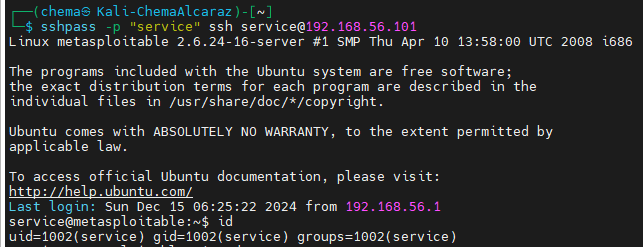
\includegraphics[width=0.5\linewidth]{img/service.png}
\end{figure}

\textbf{Recomendación:}  
\begin{itemize}
    \item Cambiar la contraseña de la cuenta \texttt{service} por una contraseña robusta.
    \item Deshabilitar la cuenta si no es necesaria.
    \item Configurar políticas de contraseñas seguras.
\end{itemize}
\newpage
\newsection{Contraseña por defecto en cuenta \texttt{user} (Crítica)}

\begin{table}[H]
\renewcommand{\arraystretch}{1.5}
\small
\centering
\begin{tabular}{|p{3.5cm}|p{2.5cm}|p{8cm}|}
\hline
\rowcolor{heading-grey}
\textbf{\textcolor{white}{Gravedad}} & \textbf{\textcolor{white}{CVSS}} & \textbf{\textcolor{white}{Descripción}} \\ \hline
\cellcolor{Critical}\textbf{\textcolor{white}{Crítica}} & 9.0 & La cuenta \texttt{user} utiliza una contraseña por defecto (\texttt{"user"}), lo que permite a un atacante obtener acceso remoto y escalar privilegios en el sistema. \\ \hline
\end{tabular}
\end{table}

\textbf{Descripción:}  
La cuenta \texttt{user} utiliza una contraseña por defecto preconfigurada (\texttt{"user"}). Esta vulnerabilidad facilita que un atacante obtenga acceso al sistema a través del servicio Telnet (puerto 23).

\textbf{Impacto:}  
El acceso no autorizado a la cuenta permite al atacante ejecutar comandos en el sistema, acceder a datos sensibles y realizar escalada de privilegios.

\textbf{Evidencia:}  
Salida del comando:  
\begin{verbatim}
telnet 192.168.56.101
\end{verbatim}
Autenticación exitosa utilizando la contraseña por defecto \texttt{user}.
\begin{figure}[H]
    \centering
    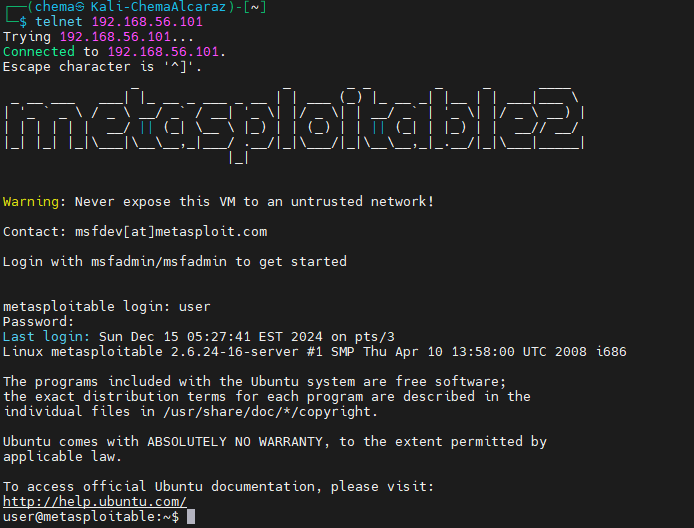
\includegraphics[width=0.5\linewidth]{img/image.png}
\end{figure}

\textbf{Recomendación:}  
\begin{itemize}
    \item Cambiar la contraseña de la cuenta \texttt{user} por una contraseña robusta.
    \item Deshabilitar la cuenta si no es necesaria.
    \item Configurar políticas de contraseñas seguras.
\end{itemize}
\newpage

\newsection{Servidor VNC con contraseña débil ("password") (Crítica)}

\begin{table}[h]
    \renewcommand{\arraystretch}{1.5} % Aumenta el espaciado en la tabla
    \begin{center}
        \begin{tabular}{|m{3.5cm}|m{2.5cm}|m{8cm}|}
            \hline
            \rowcolor{heading-grey}
            \textbf{\textcolor{white}{Gravedad}} & 
            \textbf{\textcolor{white}{CVSS}} & 
            \textbf{\textcolor{white}{Descripción}} \\ \hline
            \cellcolor{Critical}\textbf{\textcolor{white}{Crítica}} & 
            \centering 10.0 & 
            El servidor VNC permite autenticación con una contraseña débil ("password"). Esto podría permitir a un atacante tomar control completo del sistema afectado. \\ \hline
        \end{tabular}
    \end{center}
\end{table}

\textbf{Descripción:}  
Se detectó que el servidor VNC en el puerto \textbf{5900/tcp} utiliza una contraseña predeterminada débil ("password"), que no cumple con los estándares básicos de seguridad. Esta vulnerabilidad permite a un atacante remoto autenticarse sin dificultad y tomar control del sistema. El servidor VNC vulnerable fue identificado en el host \textbf{192.168.56.101}.

\textbf{Impacto:}  
La explotación de esta vulnerabilidad puede resultar en el control remoto completo del sistema afectado, comprometiendo la confidencialidad, integridad y disponibilidad de los datos. Un atacante podría usar este acceso para instalar malware, exfiltrar información sensible o realizar actividades maliciosas en la red.

\textbf{Evidencia:}  
Se obtuvo acceso al servidor VNC utilizando la contraseña predeterminada ("password") con herramientas como \texttt{Nmap} y \texttt{vncviewer}.
\begin{figure}[H]
    \centering
    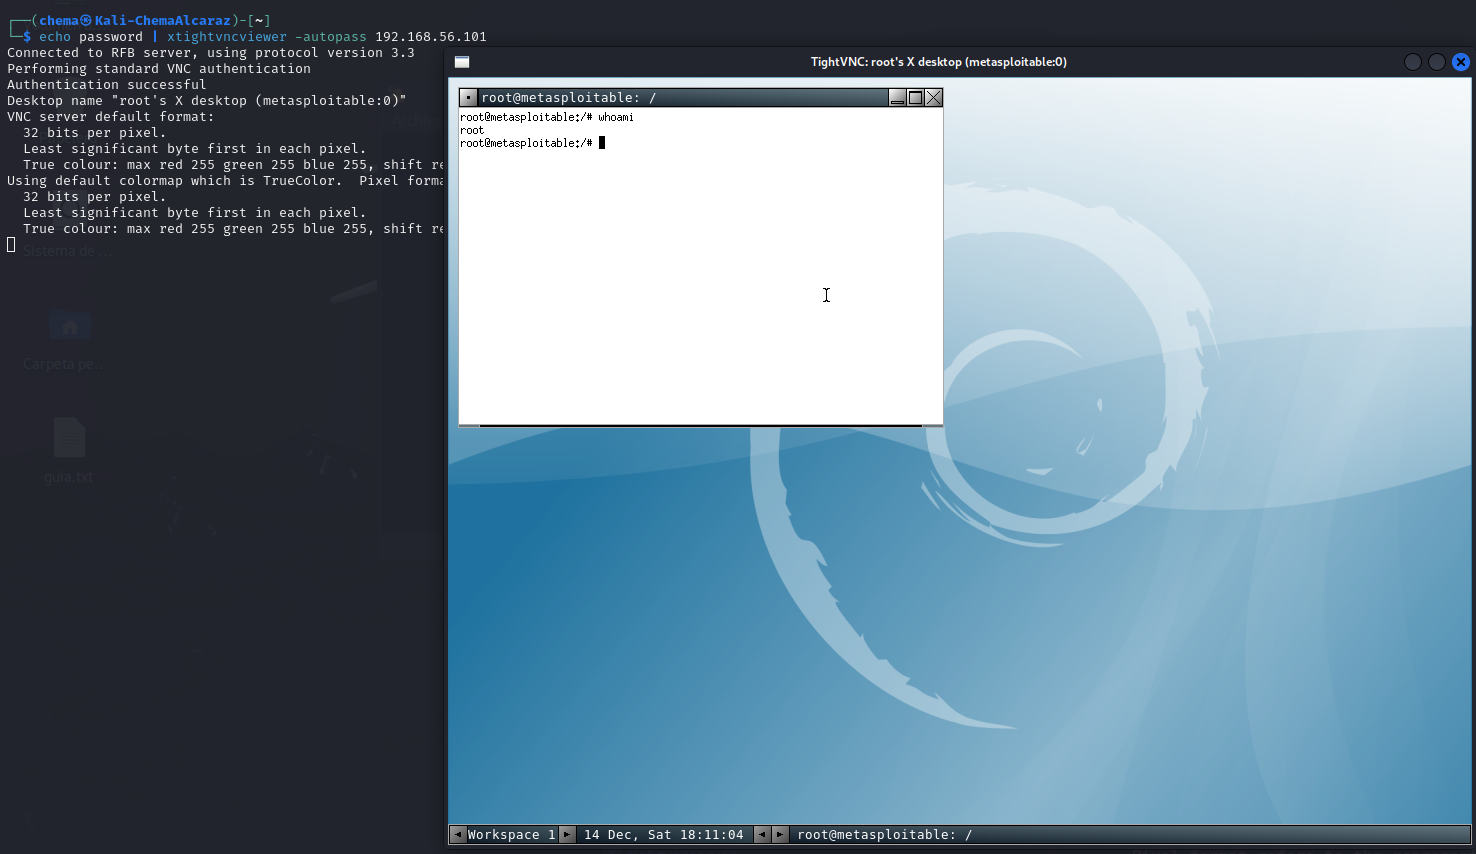
\includegraphics[width=0.5\linewidth]{img/vnc.png}
\end{figure}

\textbf{Recomendación:}  
\begin{itemize}
    \item Cambiar inmediatamente la contraseña del servidor VNC por una contraseña segura, que cumpla con los estándares de complejidad (mínimo 12 caracteres, con mezcla de letras, números y símbolos).
    \item Deshabilitar las cuentas con contraseñas predeterminadas o débiles.
    \item Configurar controles de acceso adicionales, como la autenticación basada en certificados o listas de control de acceso (ACL).
    \item Implementar mecanismos de monitoreo para detectar accesos no autorizados al servidor VNC.
\end{itemize}

\newpage
\newsection{Backdoor activo en Bind Shell (Crítica)}

\begin{table}[h]
    \renewcommand{\arraystretch}{1.5} % Aumenta el espaciado en la tabla
    \begin{center}
        \begin{tabular}{|m{3.5cm}|m{2.5cm}|m{8cm}|}
            \hline
            \rowcolor{heading-grey}
            \textbf{\textcolor{white}{Gravedad}} & 
            \textbf{\textcolor{white}{CVSS}} & 
            \textbf{\textcolor{white}{Descripción}} \\ \hline
            \cellcolor{Critical}\textbf{\textcolor{white}{Crítica}} & 
            \centering 10.0 & 
            Se detectó un backdoor activo en el puerto \textbf{1524/tcp}, permitiendo a un atacante acceder remotamente con privilegios de root sin autenticación. \\ \hline
        \end{tabular}
    \end{center}
\end{table}

\textbf{Descripción:}  
Un atacante puede explotar esta vulnerabilidad para obtener acceso remoto al sistema mediante un shell activo (bind shell) en el puerto \textbf{1524/tcp}. Este tipo de backdoor fue instalado probablemente como resultado de un compromiso previo y brinda acceso administrativo al sistema comprometido.

\textbf{Impacto:}  
La presencia de este backdoor pone en grave riesgo la seguridad del sistema y de toda la red asociada. Un atacante puede:
\begin{itemize}
    \item Ejecutar comandos con privilegios de root.
    \item Instalar malware o herramientas maliciosas adicionales.
    \item Acceder, modificar o eliminar información crítica.
    \item Usar el sistema como un punto de entrada para comprometer otros dispositivos en la red.
\end{itemize}

\textbf{Evidencia:}  
Durante el escaneo, se detectó la presencia de un servicio activo en el puerto \textbf{1524/tcp}, identificado como un shell remoto accesible sin autenticación.

\begin{figure}[H]
    \centering
    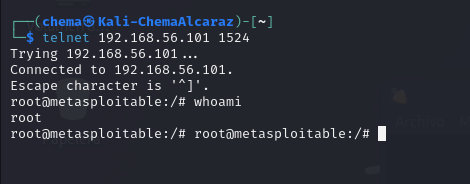
\includegraphics[width=0.5\linewidth]{img/backdoor.png}
\end{figure}

\textbf{Recomendación:}  
\begin{itemize}
    \item Cerrar inmediatamente el puerto \textbf{1524/tcp} en el firewall para evitar accesos no autorizados.
    \item Analizar el sistema para detectar otros backdoors o herramientas maliciosas.
    \item Reinstalar el sistema operativo afectado desde una fuente confiable para garantizar la eliminación completa del backdoor.
    \item Implementar medidas de detección de intrusiones (IDS) y monitoreo de tráfico para identificar actividades sospechosas.
    \item Revisar y fortalecer las políticas de acceso remoto y autenticación.
\end{itemize}

\newpage
\newsection{Backdoor en vsftpd 2.3.4 (Crítica)}

\begin{table}[h]
    \renewcommand{\arraystretch}{1.5} % Aumenta el espaciado en la tabla
    \begin{center}
        \begin{tabular}{|m{3.5cm}|m{2.5cm}|m{8cm}|}
            \hline
            \rowcolor{heading-grey}
            \textbf{\textcolor{white}{Gravedad}} & 
            \textbf{\textcolor{white}{CVSS}} & 
            \textbf{\textcolor{white}{Descripción}} \\ \hline
            \cellcolor{Critical}\textbf{Crítica} & 
            \centering 9.8 & 
            La versión de \texttt{vsftpd 2.3.4} contiene una puerta trasera que permite abrir una shell de escucha en el puerto \texttt{6200} enviando un nombre de usuario específico. \\ \hline
        \end{tabular}
    \end{center}
\end{table}

\textbf{Descripción:}  
La versión \texttt{vsftpd 2.3.4} del servidor FTP contiene una puerta trasera introducida por un atacante desconocido en el código fuente original. Si se envía un nombre de usuario que termine en el carácter `\texttt{:)}', el servicio abrirá una shell de escucha en el puerto \texttt{6200} permitiendo la ejecución remota de comandos como el usuario \textbf{root}.

\textbf{Impacto:}  
Un atacante no autenticado puede obtener acceso completo al sistema como usuario \textbf{root}, comprometiendo la confidencialidad, integridad y disponibilidad del sistema.

\textbf{Evidencia:}  
\begin{verbatim}
# telnet 192.168.56.101 21
Trying 192.168.56.101...
Connected to 192.168.56.101.
Escape character is '^]'.
220 (vsFTPd 2.3.4)
user chema:)
331 Please specify the password.
pass invalid
^]
telnet> quit
Connection closed.

# telnet 192.168.56.101 6200
Trying 192.168.56.101...
Connected to 192.168.56.101.
Escape character is '^]'.
id;
uid=0(root) gid=0(root)
\end{verbatim}

\textbf{Recomendación:}  
\begin{itemize}
    \item \textbf{Actualizar} la versión de \texttt{vsftpd} a la última versión estable disponible que no contenga esta vulnerabilidad.
    \item \textbf{Verificar} la integridad del código fuente o de los binarios descargados para evitar versiones comprometidas.
    \item \textbf{Monitorear y restringir} el acceso al puerto 21 y 6200 mediante un firewall o políticas de red.
    \item \textbf{Deshabilitar temporalmente} el servicio FTP si no es absolutamente necesario.
\end{itemize}


\newpage
\newsection{phpMyAdmin vulnerable a inyecciones SQL (Crítica)}

\begin{table}[h]
    \renewcommand{\arraystretch}{1.5} % Aumenta el espaciado en la tabla
    \begin{center}
        \begin{tabular}{|m{3.5cm}|m{2.5cm}|m{8cm}|}
            \hline
            \rowcolor{heading-grey}
            \textbf{\textcolor{white}{Gravedad}} & 
            \textbf{\textcolor{white}{CVSS}} & 
            \textbf{\textcolor{white}{Descripción}} \\ \hline
            \cellcolor{Critical}\textbf{\textcolor{white}{Crítica}} & 
            \centering 9.8 & 
            phpMyAdmin en versiones anteriores a \textbf{4.8.6} es vulnerable a inyecciones SQL, exponiendo datos sensibles o permitiendo modificaciones arbitrarias en la base de datos. \\ \hline
        \end{tabular}
    \end{center}
\end{table}

\textbf{Descripción:}  
El servicio phpMyAdmin en el puerto \textbf{80/tcp} se encontró en una versión obsoleta (\textbf{3.1.1}), conocida por ser vulnerable a inyecciones SQL (SQLi). Esta vulnerabilidad permite a un atacante enviar consultas SQL maliciosas al servidor, comprometiendo la confidencialidad e integridad de la base de datos.

\textbf{Impacto:}  
Un atacante puede explotar esta vulnerabilidad para:
\begin{itemize}
    \item Acceder a información sensible almacenada en la base de datos (e.g., contraseñas, datos de usuarios, etc.).
    \item Modificar o eliminar registros críticos.
    \item Obtener acceso administrativo al servidor de la base de datos.
    \item Escalar privilegios para comprometer otros servicios conectados.
\end{itemize}

\textbf{Evidencia:}  
El escaneo identificó phpMyAdmin ejecutándose en la versión \textbf{3.1.1}, que es anterior a la versión segura \textbf{4.8.6}.

Sin evidencia grafica. Link a CVE: \href{https://nvd.nist.gov/vuln/detail/CVE-2019-11768}{CVE-2019-11768}

\textbf{Recomendación:}  
\begin{itemize}
    \item Actualizar phpMyAdmin a la última versión disponible (4.8.6 o superior).
    \item Restringir el acceso al servicio phpMyAdmin mediante listas de control de acceso (ACL).
    \item Configurar parámetros seguros en el servidor de la base de datos, como limitar usuarios con permisos administrativos.
    \item Monitorear y registrar las actividades en el servicio phpMyAdmin para detectar posibles intentos de explotación.
\end{itemize}

\newpage
\newsection{PHP-CGI permite ejecución remota de comandos (Crítica)}

\begin{table}[h]
    \renewcommand{\arraystretch}{1.5} % Aumenta el espaciado en la tabla
    \begin{center}
        \begin{tabular}{|m{3.5cm}|m{2.5cm}|m{8cm}|}
            \hline
            \rowcolor{heading-grey}
            \textbf{\textcolor{white}{Gravedad}} & 
            \textbf{\textcolor{white}{CVSS}} & 
            \textbf{\textcolor{white}{Descripción}} \\ \hline
            \cellcolor{Critical}\textbf{\textcolor{white}{Crítica}} & 
            \centering 9.8 & 
            Una configuración insegura en PHP-CGI permite a un atacante pasar argumentos arbitrarios y ejecutar comandos en el sistema afectado. \\ \hline
        \end{tabular}
    \end{center}
\end{table}

\textbf{Descripción:}  
El servidor web que opera en el puerto \textbf{80/tcp} contiene una instalación vulnerable de \textbf{PHP-CGI} que permite a un atacante remoto ejecutar comandos arbitrarios en el sistema. Esta vulnerabilidad se produce debido a que el parámetro de consulta puede manipularse para enviar argumentos de línea de comandos directamente a PHP.

\textbf{Impacto:}  
Un atacante puede explotar esta vulnerabilidad para:
\begin{itemize}
    \item Ejecutar comandos con los mismos privilegios que el usuario del servidor web.
    \item Comprometer la seguridad del sistema completo.
    \item Exfiltrar datos sensibles almacenados en el servidor.
    \item Instalar malware o persistencias maliciosas en el servidor afectado.
\end{itemize}

\textbf{Evidencia:}  
Se detectó una versión vulnerable de PHP-CGI configurada en el servidor web.
\begin{figure}[H]
    \centering
    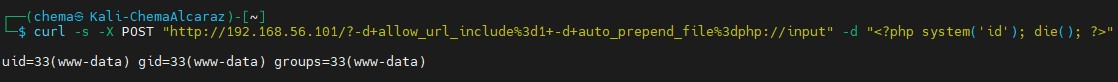
\includegraphics[width=1\linewidth]{img/php-cgi.jpg}
\end{figure}

\textbf{Recomendación:}  
\begin{itemize}
    \item Actualizar PHP-CGI a una versión más reciente que no esté afectada por esta vulnerabilidad (recomendado: 5.3.13 o superior).
    \item Revisar la configuración del servidor web para asegurarse de que no se permiten parámetros arbitrarios en el intérprete PHP.
    \item Implementar restricciones en el acceso al servidor web para evitar intentos de explotación.
    \item Monitorear y registrar las actividades del servidor para detectar intentos de explotación.
\end{itemize}

\newpage
\newsection{Servicio rlogin transmite datos en texto claro (Crítica)}

\begin{table}[h]
    \renewcommand{\arraystretch}{1.5} % Aumenta el espaciado en la tabla
    \begin{center}
        \begin{tabular}{|m{3.5cm}|m{2.5cm}|m{8cm}|}
            \hline
            \rowcolor{heading-grey}
            \textbf{\textcolor{white}{Gravedad}} & 
            \textbf{\textcolor{white}{CVSS}} & 
            \textbf{\textcolor{white}{Descripción}} \\ \hline
            \cellcolor{Critical}\textbf{\textcolor{white}{Crítica}} &  
            \centering 9.8 & 
            El servicio rlogin en el puerto \textbf{513/tcp} transmite datos, incluidas credenciales, en texto claro, exponiéndolos a posibles ataques de interceptación. \\ \hline
        \end{tabular}
    \end{center}
\end{table}

\textbf{Descripción:}  
El servicio rlogin detectado en el puerto \textbf{513/tcp} permite a los usuarios autenticarse y acceder remotamente al sistema. Sin embargo, este protocolo transmite los datos en texto claro, lo que lo hace vulnerable a ataques de tipo "man-in-the-middle" y permite que un atacante intercepte credenciales o comandos.

\textbf{Impacto:}  
Un atacante que intercepte el tráfico rlogin podría:
\begin{itemize}
    \item Obtener credenciales de usuarios en texto claro.
    \item Suplantar la identidad de usuarios legítimos y acceder al sistema afectado.
    \item Ejecutar comandos maliciosos en el sistema con los privilegios del usuario autenticado.
    \item Comprometer la confidencialidad de la comunicación entre el cliente y el servidor.
\end{itemize}

\textbf{Evidencia:}  
Durante el escaneo, se identificó el servicio rlogin en el puerto \textbf{513/tcp}.
\begin{figure}[H]
    \centering
    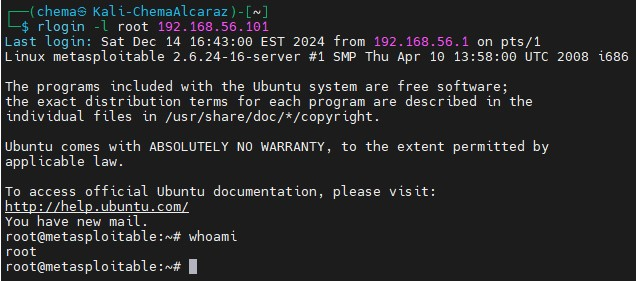
\includegraphics[width=0.7\linewidth]{img/rlogin.jpg}
\end{figure}

\textbf{Recomendación:}  
\begin{itemize}
    \item Deshabilitar inmediatamente el servicio rlogin en el sistema afectado.
    \item Configurar \textbf{SSH} como alternativa segura para accesos remotos.
    \item Actualizar las políticas de acceso remoto para prohibir el uso de protocolos no cifrados.
    \item Implementar reglas en el firewall para bloquear conexiones al puerto \textbf{513/tcp}.
    \item Monitorear la red en busca de intentos de conexión al servicio rlogin.
\end{itemize}

\newpage
\newsection{Badlock en Samba permite ataques man-in-the-middle (Alta)}

\begin{table}[h]
    \renewcommand{\arraystretch}{1.5} % Aumenta el espaciado en la tabla
    \begin{center}
        \begin{tabular}{|m{3.5cm}|m{2.5cm}|m{8cm}|}
            \hline
            \rowcolor{heading-grey}
            \textbf{\textcolor{white}{Gravedad}} & 
            \textbf{\textcolor{white}{CVSS}} & 
            \textbf{\textcolor{white}{Descripción}} \\ \hline
            \cellcolor{High}\textbf{Alta} & 
            \centering 7.8 & 
            La vulnerabilidad Badlock en Samba permite a un atacante realizar ataques man-in-the-middle para interceptar y modificar el tráfico entre clientes y servidores. \\ \hline
        \end{tabular}
    \end{center}
\end{table}

\textbf{Descripción:}  
El servicio Samba identificado en los puertos \textbf{139/tcp} y \textbf{445/tcp} contiene una vulnerabilidad conocida como \textbf{Badlock}, que afecta la autenticación de SMB. Este fallo permite a un atacante interceptar el tráfico de la red y, en algunos casos, reducir el nivel de seguridad del protocolo para manipular llamadas SMB.

\textbf{Impacto:}  
Un atacante puede explotar esta vulnerabilidad para:
\begin{itemize}
    \item Interceptar credenciales de usuarios en tránsito.
    \item Modificar el contenido del tráfico SMB para comprometer datos.
    \item Realizar ataques de tipo "replay" para suplantar usuarios legítimos.
    \item Escalar privilegios dentro del sistema comprometido.
\end{itemize}

\textbf{Evidencia:}  
Durante el escaneo, se identificó el servicio Samba con soporte SMB en los puertos \textbf{139/tcp} y \textbf{445/tcp}.
\begin{figure}[H]
    \centering
    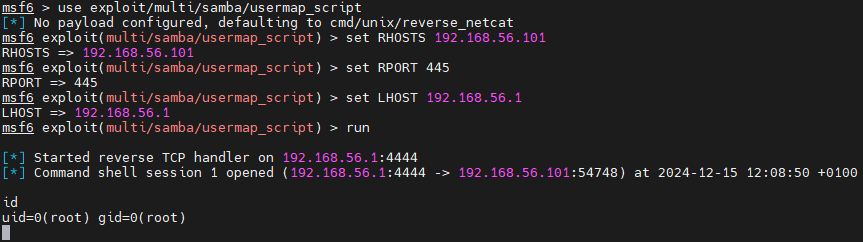
\includegraphics[width=0.5\linewidth]{img/samba.png}
\end{figure}

\textbf{Recomendación:}  
\begin{itemize}
    \item Actualizar Samba a las versiones seguras (4.2.11, 4.3.8 o 4.4.2 o superiores).
    \item Configurar SMB para requerir autenticación fuerte y cifrada.
    \item Deshabilitar versiones antiguas del protocolo SMB (e.g., SMBv1).
    \item Implementar medidas de monitoreo para detectar actividades sospechosas relacionadas con SMB.
    \item Establecer reglas de firewall que limiten el acceso a los puertos \textbf{139/tcp} y \textbf{445/tcp} solo a hosts confiables.
\end{itemize}

\newpage
\newsection{Acceso no restringido a recursos compartidos NFS (Alta)}

\begin{table}[h]
    \renewcommand{\arraystretch}{1.5} % Aumenta el espaciado en la tabla
    \begin{center}
        \begin{tabular}{|m{3.5cm}|m{2.5cm}|m{8cm}|}
            \hline
            \rowcolor{heading-grey}
            \textbf{\textcolor{white}{Gravedad}} & 
            \textbf{\textcolor{white}{CVSS}} & 
            \textbf{\textcolor{white}{Descripción}} \\ \hline
            \cellcolor{High}\textbf{Alta} & 
            \centering 7.5 & 
            El servidor NFS en el puerto \textbf{2049/tcp} permite acceso no restringido a recursos compartidos, exponiendo información sensible y aumentando el riesgo de manipulación no autorizada. \\ \hline
        \end{tabular}
    \end{center}
\end{table}

\textbf{Descripción:}  
El servicio NFS (Network File System) en el puerto \textbf{2049/tcp} permite que usuarios no autenticados accedan a recursos compartidos sin restricciones de acceso adecuadas. Esto representa un grave riesgo para la confidencialidad y la integridad de los datos almacenados en el sistema.

\textbf{Impacto:}  
Un atacante podría explotar esta vulnerabilidad para:
\begin{itemize}
    \item Acceder y leer datos sensibles almacenados en los recursos compartidos NFS.
    \item Modificar o eliminar archivos en los recursos compartidos sin autorización.
    \item Realizar movimientos laterales dentro de la red utilizando los datos comprometidos.
    \item Utilizar los recursos compartidos como punto de apoyo para ataques más amplios en la infraestructura.
\end{itemize}

\textbf{Evidencia:}  
Durante el escaneo, se identificó que el servidor NFS en el puerto \textbf{2049/tcp} estaba exportando recursos compartidos sin aplicar restricciones de acceso (e.g., por dirección IP o rango de red).
\begin{figure}[H]
    \centering
    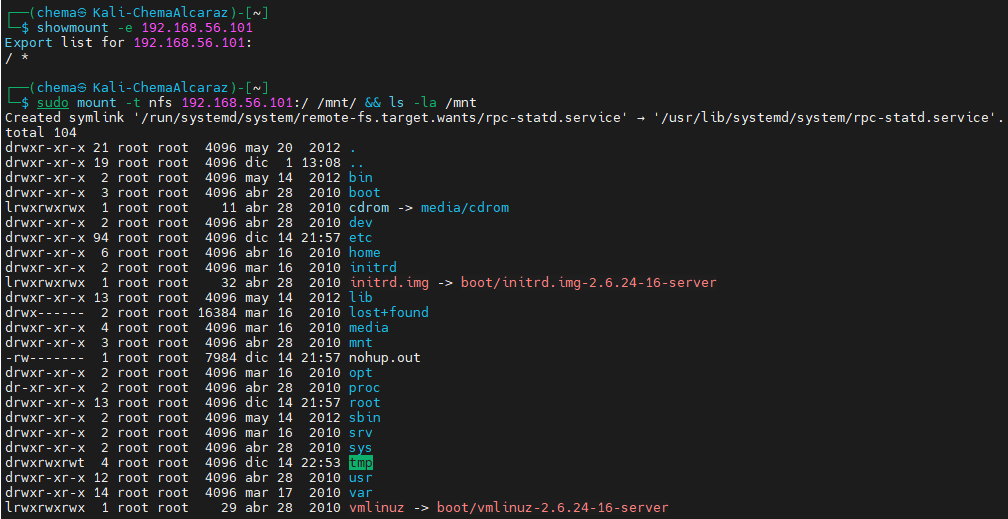
\includegraphics[width=0.5\linewidth]{img/nfs.png}
\end{figure}

\textbf{Recomendación:}  
\begin{itemize}
    \item Configurar las restricciones de acceso en el servidor NFS utilizando listas de control de acceso basadas en IP (hosts.allow/hosts.deny).
    \item Limitar los permisos de escritura en los recursos compartidos a usuarios específicos.
    \item Habilitar el cifrado en las conexiones NFS para proteger los datos en tránsito.
    \item Monitorizar el acceso a los recursos compartidos NFS para detectar actividades sospechosas.
\end{itemize}

\newpage
\newsection{TWiki permite ejecución remota de comandos (Alta)}

\begin{table}[h]
    \renewcommand{\arraystretch}{1.5} % Aumenta el espaciado en la tabla
    \begin{center}
        \begin{tabular}{|m{3.5cm}|m{2.5cm}|m{8cm}|}
            \hline
            \rowcolor{heading-grey}
            \textbf{\textcolor{white}{Gravedad}} & 
            \textbf{\textcolor{white}{CVSS}} & 
            \textbf{\textcolor{white}{Descripción}} \\ \hline
            \cellcolor{High}\textbf{Alta} & 
            \centering 8.8 & 
            TWiki permite a un atacante manipular el parámetro `rev` para ejecutar comandos arbitrarios en el servidor afectado. \\ \hline
        \end{tabular}
    \end{center}
\end{table}

\textbf{Descripción:}  
El servicio web que opera en el puerto \textbf{80/tcp} incluye una versión vulnerable de TWiki, un software de gestión de contenido. Esta vulnerabilidad permite a un atacante ejecutar comandos del sistema a través de la manipulación del parámetro `rev` en las solicitudes HTTP, comprometiendo el servidor.

\textbf{Impacto:}  
Un atacante podría explotar esta vulnerabilidad para:
\begin{itemize}
    \item Ejecutar comandos arbitrarios en el servidor con los privilegios del usuario del servidor web.
    \item Exfiltrar datos sensibles almacenados en el servidor.
    \item Escalar privilegios para comprometer el sistema completo.
    \item Instalar malware o persistencias en el servidor afectado.
\end{itemize}

\textbf{Evidencia:}  
Durante el análisis, se detectó una vulnerabilidad en el parámetro `rev` de TWiki, permitiendo la ejecución remota de comandos.
\begin{figure}[H]
    \centering
    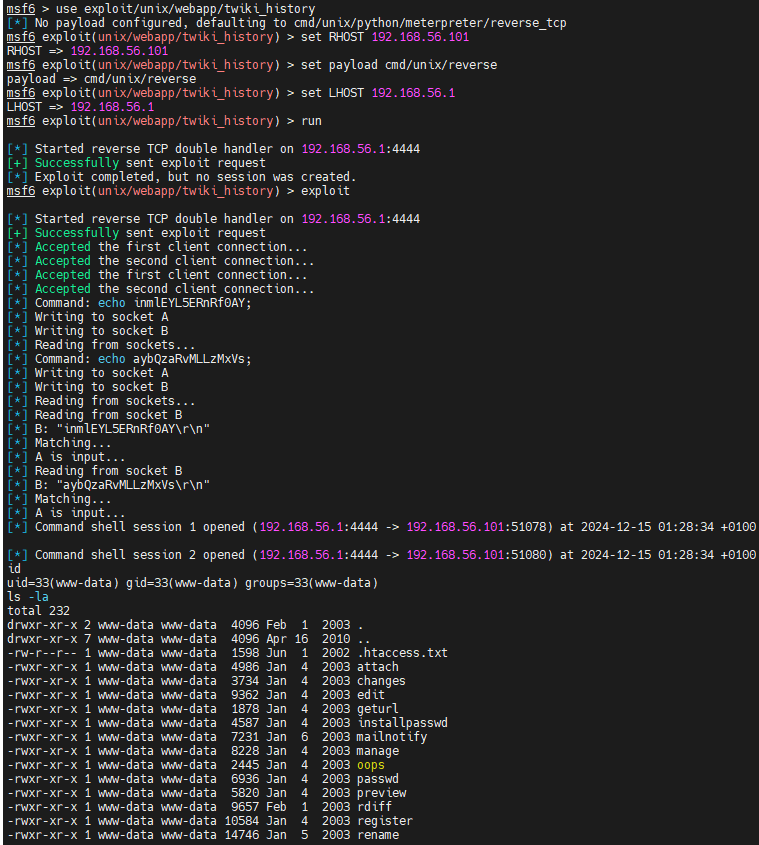
\includegraphics[width=0.5\linewidth]{img/twiki.png}
\end{figure}
\newpage
\textbf{Recomendación:}  
\begin{itemize}
    \item Actualizar TWiki a la versión más reciente que no esté afectada por esta vulnerabilidad.
    \item Restringir el acceso al servicio TWiki mediante controles de acceso basados en IP.
    \item Monitorear el tráfico HTTP hacia el servidor para detectar patrones maliciosos.
    \item Aplicar políticas de validación de entradas en el servidor para evitar inyecciones y manipulaciones de parámetros.
\end{itemize}

\newpage
\newsection{Apache Tomcat versión obsoleta con múltiples vulnerabilidades (Crítica)}

\begin{table}[h]
    \renewcommand{\arraystretch}{1.5} % Aumenta el espaciado en la tabla
    \begin{center}
        \begin{tabular}{|m{3.5cm}|m{2.5cm}|m{8cm}|}
            \hline
            \rowcolor{heading-grey}
            \textbf{\textcolor{white}{Gravedad}} & 
            \textbf{\textcolor{white}{CVSS}} & 
            \textbf{\textcolor{white}{Descripción}} \\ \hline
            \cellcolor{Critical}\textbf{\textcolor{white}{Crítica}} & 
            \centering 9.8 & 
            La versión de Apache Tomcat instalada (\textless= 5.5.x) ha alcanzado su fin de vida útil, dejando múltiples vulnerabilidades sin parchear. \\ \hline
        \end{tabular}
    \end{center}
\end{table}

\textbf{Descripción:}  
El servicio Apache Tomcat identificado en el puerto \textbf{8180/tcp} está ejecutándose en una versión obsoleta que ya no recibe soporte ni actualizaciones de seguridad. Esto lo hace susceptible a vulnerabilidades conocidas y desconocidas.

\textbf{Impacto:}  
Un atacante puede aprovechar las vulnerabilidades de esta versión para:
\begin{itemize}
    \item Obtener acceso remoto al servidor.
    \item Comprometer aplicaciones web desplegadas en Tomcat.
    \item Escalar privilegios en el sistema afectado.
    \item Realizar ataques de denegación de servicio (DoS).
\end{itemize}

\textbf{Evidencia:}  
Se identificó que Apache Tomcat ejecuta una versión anterior a 5.5.x, que es vulnerable a múltiples fallos críticos.


\textbf{Recomendación:}  
\begin{itemize}
    \item Actualizar Apache Tomcat a una versión soportada, como 9.x o superior.
    \item Revisar todas las aplicaciones web desplegadas en el servidor para verificar su integridad.
    \item Configurar reglas de firewall para restringir el acceso al puerto \textbf{8180/tcp} solo a hosts confiables.
    \item Monitorear continuamente el servidor en busca de intentos de explotación.
\end{itemize}


\newpage
\newsection{Conector AJP vulnerable a Ghostcat (Crítica)}

\begin{table}[h]
    \renewcommand{\arraystretch}{1.5} % Aumenta el espaciado en la tabla
    \begin{center}
        \begin{tabular}{|m{3.5cm}|m{2.5cm}|m{8cm}|}
            \hline
            \rowcolor{heading-grey}
            \textbf{\textcolor{white}{Gravedad}} & 
            \textbf{\textcolor{white}{CVSS}} & 
            \textbf{\textcolor{white}{Descripción}} \\ \hline
            \cellcolor{Critical}\textbf{\textcolor{white}{Crítica}} & 
            \centering 9.8 & 
            Vulnerabilidad "Ghostcat" en el conector AJP de Apache Tomcat que permite lectura de archivos y ejecución remota de código. \\ \hline
        \end{tabular}
    \end{center}
\end{table}

\textbf{Descripción:}  
El conector AJP identificado en el puerto \textbf{8009/tcp} es vulnerable a la explotación conocida como \textbf{Ghostcat}. Esto permite a un atacante remoto acceder a archivos confidenciales del servidor y, en ciertos casos, ejecutar código arbitrario.

\textbf{Impacto:}  
Un atacante podría:
\begin{itemize}
    \item Leer archivos confidenciales desde el servidor, incluyendo configuraciones críticas.
    \item Subir archivos maliciosos para obtener ejecución remota de código.
    \item Comprometer aplicaciones web alojadas en el servidor Apache Tomcat.
    \item Escalar privilegios dentro del sistema comprometido.
\end{itemize}

\textbf{Evidencia:}  
Se identificó la presencia del conector AJP en el puerto \textbf{8009/tcp}, junto con configuraciones vulnerables explotables por Ghostcat.

\textbf{Recomendación:}  
\begin{itemize}
    \item Actualizar Apache Tomcat a una versión segura (7.0.100, 8.5.51, 9.0.31 o superior).
    \item Deshabilitar el conector AJP si no es estrictamente necesario.
    \item Configurar autenticación para proteger el acceso al conector AJP.
    \item Monitorear los logs de acceso de Tomcat para identificar actividades sospechosas.
\end{itemize}



\end{document}
